Este capítulo tem como objetivo apresentar a metodologia da avaliação de desempenho das diferentes bibliotecas de ML selecionadas.

\section{Motivação}%
\label{3-motivation}

Avaliações são importantes na busca pelo máximo desempenho de um sistema com os recursos disponíveis. Seus resultados auxiliam tanto nas decisões de escolhas entre diferentes sistemas ou simplesmente entender o funcionamento de um sistema já existente. Devido à grande diversidade de sistemas, não existe um procedimento padrão comum em que seja possível analisar eficientemente um sistema qualquer, sendo necessário conhecer o sistema a ser avaliado e escolher as métricas, carga de trabalho e técnicas de avaliação apropriadas. \cite{jain1991art}

Uma simulação executada por simuladores de EONs costuma envolver dezenas de milhares de eventos como requisições de conexões. Tamanha magnitude do número de eventos representa a importância de um bom desempenho na execução de modelos, como por exemplo em propostas de soluções para problemas de alocação de recursos (e.g. RSA) cujos modelos seriam executados em cada evento.

Assim, uma análise quantitativa do desempenho de bibliotecas de ML é importante na busca por uma solução de integração de ML com simuladores que seja flexível de acordo com as necessidades de cada pesquisa e que possua um bom desempenho de modo a acelerar a obtenção de resultados.

\section{Metodologia}%
\label{3-methodology}

De acordo com Raj Jain \cite{jain1991art}, há três métodos de avaliação de desempenho: modelagem analítica, simulação e medição. O sistema a ser avaliado, devido à presença de modelos de redes neurais profundas, é complexo o suficiente para tornar a modelagem analítica inviável. A medição foi descartada pelo fato de não buscar-se uma solução para apenas um simulador e haver um alto custo de implementação para cada possibilidade de integração. Por estes motivos, os resultados serão obtidos por meio de simulações.

\subsection{Ambiente de Simulação}

Para a realização da simulação, 10 programas foram desenvolvidos considerando todas as combinações de linguagens (Java e Python), bibliotecas (ONNX Runtime, Tensorflow Lite, Tensorflow, OpenCV e Deeplearning4j) e o uso ou não da GPU para execução de modelos. Estes programas realizam o mesmo conjunto de tarefas: 1. carregar o modelo e inicializar procedimentos necessários para futuras execuções; 2. carregar a carga de trabalho usada como entrada do modelo; 3. executar o modelo com as entradas carregadas.

Cada programa trata de medir apenas o intervalo de tempo em que a execução do modelo ocorre, sem considerar outros fatores como o tempo de carregamento da carga de trabalho ou do modelo em si. A execução de cada instância de simulação foi orquestrada por \textit{scripts} auxiliares feitos em Python, responsáveis por instalar dependências, compilar e executar os programas de simulação.

As simulações foram realizadas em uma máquina com processador Intel Core i3-8100, placa de vídeo GeForce RTX 2060 e memória RAM de 32 GB (2x16GB 3000Mhz DDR4). O código-fonte dos programas de simulação e de programas auxiliares pode ser encontrado na url \url{tcc.mikaelmello.com}.

\subsection{Modelos e Cargas de Trabalho}

Para a simulação, um classificador de estratégias de RSA em EONs, baseado em \textit{deep learning}, será utilizado para comparação. Este modelo recebe como entrada o estado de uma EON e tem como saída a classificação da estratégia RSA em utilização, de acordo com o estado. O modelo possui como saída uma classificação da estratégia de alocação identificada pelo estado como ruim, média ou boa.

A carga de trabalho é formada por 97301 diferentes estados de rede, sendo cada estado representado por uma matriz de 86 linhas e 320 colunas, a representação da topologia USANet com 24 nós e 86 enlaces em que cada enlace contém 320 \textit{slots}.

\subsection{Métricas}

Devido à necessidade de diminuir o tempo de inferência dos modelos como elencado na seção \ref{3-motivation}, esta será a métrica de desempenho avaliada, sendo definida como o tempo total percorrido desde a chamada do serviço de execução de modelos, o método \texttt{classify} da classe \texttt{Classifier} na implementação das simulações, até o retorno da chamada.

Além disso, como a execução dos modelos em diferentes bibliotecas exigem algumas conversões do formato de serialização, será avaliado se em alguma das simulações, o resultado de execuções do modelo difere de outras simulações.

\subsection{Execução}

Foram testadas 10 combinações de linguagens, bibliotecas, uso ou não de GPU e formato do modelo executado:

\begin{itemize}
  \item Java, Deeplearning4j, sem GPU, modelo original no formato HDF5 (TensorFlow);
  \item Java, Deeplearning4j, com GPU, modelo original no formato HDF5 (TensorFlow);
  \item Java, ONNX Runtime, sem GPU, modelo convertido para o formato ONNX;
  \item Java, ONNX Runtime, com GPU, modelo convertido para o formato ONNX;
  \item Python, OpenCV, sem GPU, modelo convertido para o formato ONNX;
  \item Python, Tensorflow Lite, sem GPU, modelo convertido para o formato TFLite;
  \item Python, Tensorflow, sem GPU, modelo original no formato HDF5 (TensorFlow);
  \item Python, Tensorflow, com GPU, modelo original no formato HDF5 (TensorFlow);
  \item Python, ONNX Runtime, sem GPU, modelo convertido para o formato ONNX;
  \item Python, ONNX Runtime, com GPU, modelo convertido para o formato ONNX.
\end{itemize}

Cada elemento da carga de trabalho foi executado 5 vezes por todas as combinações de simulação, sendo selecionada a mediana de cada uma destas 5 execuções com o objetivo de remover ruídos arbitrários causados pela máquina durante a execução.

\section{Resultados}

Programas Java são popularmente conhecidos pelo seu alto tempo de inicialização que causa a desaceleração da execução de outras tarefas, como as execuções da simulação. Por este motivo, as primeiras 1000 execuções foram descartadas nesta análise geral.

De acordo com a tabela \ref{tab:all}, a execução do modelo com a biblioteca Deeplearning4j em Java é a mais rápida em média, de modo que a execução sem uso de GPU é em média 300 microsegundos mais rápida que a execução com GPU, porém possui um desvio padrão muito maior devido a diversas limitações deste caso de uso: execuções em CPU estão mais sujeitas a interrupções externas, como por exemplo o coletor de lixo da JVM ou trocas de contexto do sistema operacional.

\begin{table}
  \centering
  \begin{tabular}{lllrrrrrr}
    \toprule
           &                 &     & média   & desvio padrão & mínimo & máximo \\
    ling.  & biblioteca      & GPU &         &               &        &        \\
    \midrule
    Java   & Deeplearning4j  & sem & 765.89  & 121.34        & 722    & 14620  \\
           &                 & com & 1027.66 & 35.53         & 990    & 2180   \\
           & ONNX Runtime    & sem & 2365.80 & 153.39        & 2322   & 23961  \\
           &                 & com & 2067.71 & 12.62         & 2041   & 2383   \\
    Python & ONNX Runtime    & sem & 2105.99 & 12.30         & 2060   & 2276   \\
           &                 & com & 1767.82 & 10.62         & 1729   & 1902   \\
           & OpenCV          & sem & 1773.15 & 12.41         & 1729   & 1972   \\
           & TensorFlow      & sem & 2988.95 & 19.50         & 2940   & 3332   \\
           &                 & com & 2885.59 & 18.68         & 2827   & 3219   \\
           & TensorFlow Lite & sem & 2083.73 & 12.20         & 2043   & 2218   \\
    \bottomrule
  \end{tabular}
  \caption{Estatísticas descritivas acerca do tempo de execução (microsegundos) do modelo em todas as combinações de simulação, descartadas as primeiras 1000 execuções}
  \label{tab:all}
\end{table}

A simulação com a biblioteca ONNX Runtime, sendo a única presente em programas Java e Python, foi importante para observar o melhor desempenho de programas Python em versões que utilizam e não utilizam a GPU para inferência. Além disso, a alta variância do tempo de execução na versão em Java com uso da CPU para inferência repete o comportamento visto na execução do Deeplearning4j.

As simulações com bibliotecas da família TensorFlow mostram um desempenho expressivamente maior da biblioteca TensorFlow Lite, uma biblioteca otimizada para inferência de modelos, comparada com TensorFlow.

As simulações de ambas bibliotecas ONNX Runtime e TensorFlow mostram uma melhora de desempenho significativa ao utilizar a GPU da máquina para a execução dos modelos, com ganhos que variam de 100 a 300 microsegundos em média, ao contrário de Deeplearning4j que se mostrou mais devagar com o uso da CPU. Apesar da GPU ser em geral mais rápida na execução de modelos pelas suas características, um dos motivos para este cenário acontecer é a presença de sobrecarga adicional de tempo ao transferir dados da CPU para a GPU, mais significativa quando o tempo de execução do Deeplearning4j na CPU é em média de duas a três vezes menor comparado com as outras bibliotecas.

Também é possível observar que o tempo de execução para as combinações "Python, ONNX Runtime, sem GPU", "Python, TensorFlow Lite, sem GPU" e "Java, ONNX Runtime, com GPU" é virtualmente igual. Assim como os tempos das combinações "Python, OpenCV, sem GPU" e "Python, ONNX Runtime, com GPU", apesar deste último par possuir 300 microsegundos a menos de tempo de execução em média. Após estudos e experimentos adicionais, não foi possível achar uma explicação satisfatória para a inesperada similaridade entre combinações tão diversas.

Todas as execuções com entradas iguais para o modelo resultaram em saídas iguais, sinalizando que não houve perda ou ganho de precisão ao converter o modelo original no formato HDF5 para os formatos TFLite e ONNX.

Por fim, pode-se concluir que o uso de CPU em programas Java é suscetível a diversas interrupções, gerando uma alta variância no tempo de execução do modelo. O uso de GPU não necessariamente representa um ganho de desempenho, sendo importante observar fatores como a sobrecarga de transferência de dados. Programas Python ou que utilizam a GPU para inferência possuem uma baixa variância de tempos de execuções.

\begin{figure}[h]
  \centerline{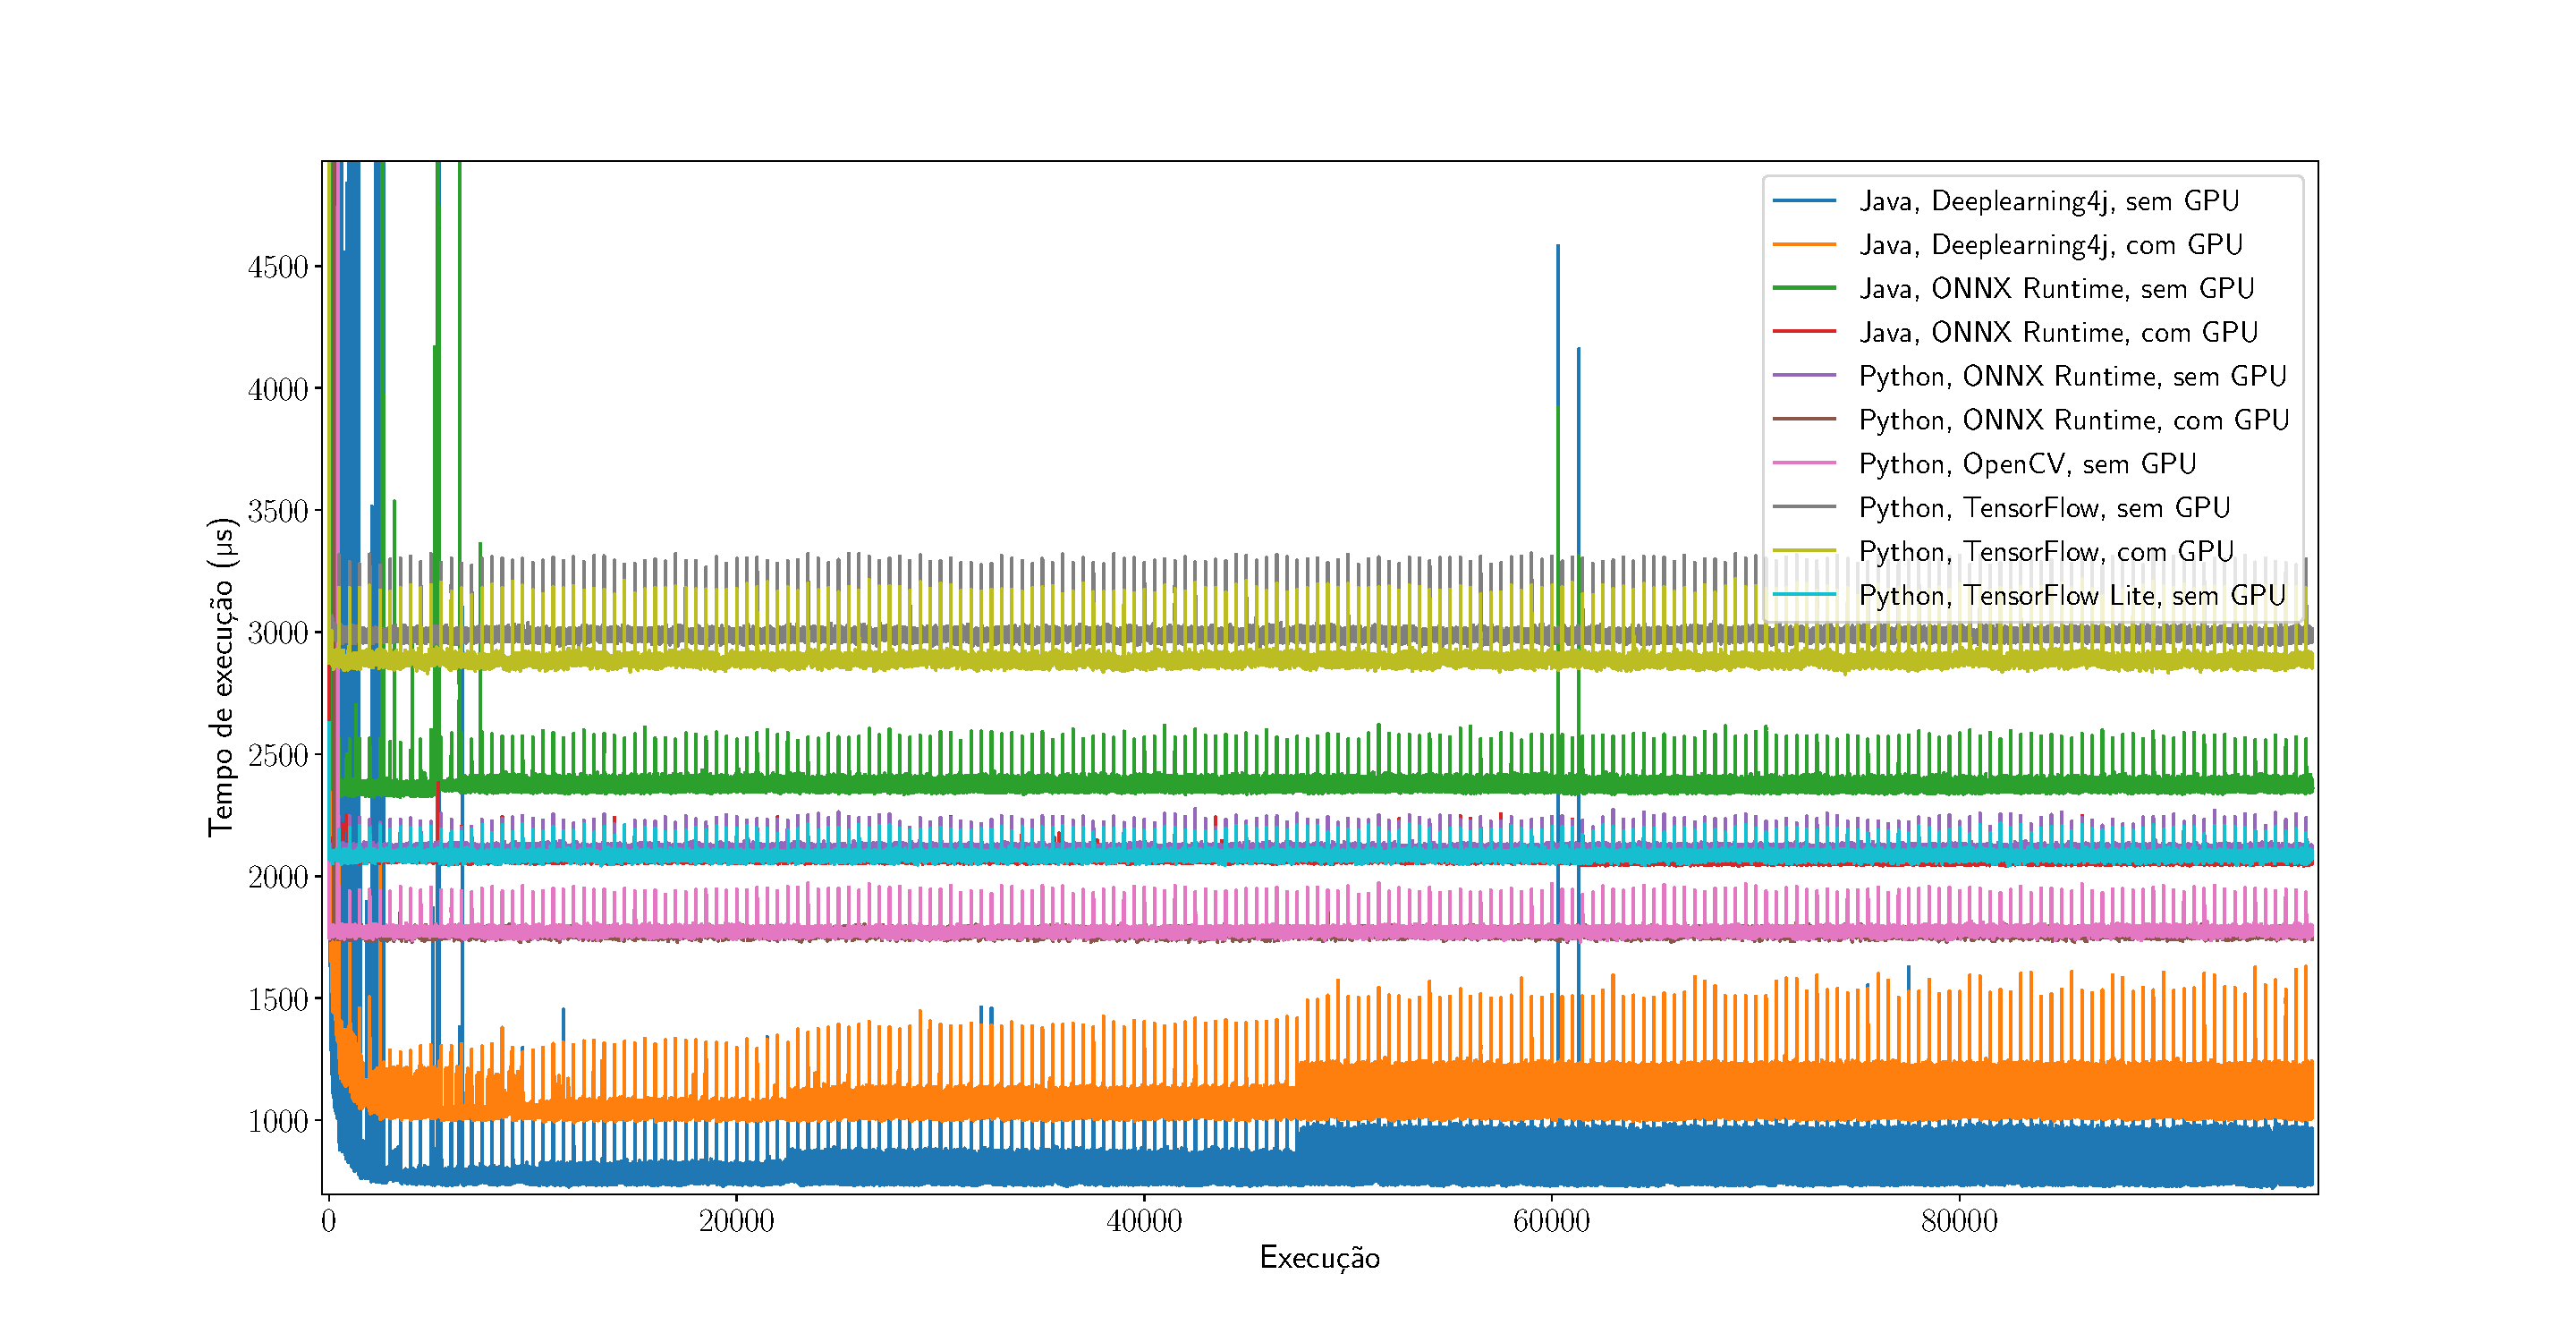
\includegraphics[width=\paperwidth]{img/all.pdf}}
  \caption{Tempo de execução de execuções sequenciais do modelo para cada programa de simulação}
  \label{fig:all}
\end{figure}